\documentclass[../../../../main.tex]{subfiles}
\begin{document}
\section*{京都大学 2001年 前期}
\begin{center}
京大理科数学 2001
\end{center}

\subsection*{第1問}
[解] $P(t, t^3)\ (t \in \mathbb{R})$ とおく。$P$ における接線 $l$ として
\[ l: y - t^3 = 3t^2(x - t) \]
である。$l$ 上の点 $(X,Y)$ が $L$ 上の点 $(x,y)$ にうつったとすると、
\begin{eqnarray*}
\{ (X-t) + i(Y-t^3) \} &=& \frac{\sqrt{2}}{2}(1-i) \{ (x-t) + i(y-t^3) \} \\
&=& \frac{\sqrt{2}}{2} \left[ \{ (x-t) + (y-t^3) \} + i \{ (y-t^3) - (x-t) \} \right] \\
&=& \frac{\sqrt{2}}{2} \left[ (x+y-t-t^3) + i (-x+y+t-t^3) \right]
\end{eqnarray*}
から
\[ X-t = \frac{\sqrt{2}}{2}(x+y-t-t^3),\ Y-t^3 = \frac{\sqrt{2}}{2}(-x+y+t-t^3)\ (x, y, X, Y, t \in \mathbb{R}) \]
だから
\[ l: -x+y+t-t^3 = 3t^2 (x+y-t-t^3) \cdots \text{\textcircled{1}} \]
これが $y=x^3$ と $3$ 異交点を持つ時、\textcircled{1} に $y=x^3$ を代入した
\begin{eqnarray*}
-x+x^3+t-t^3 &=& 3t^2 (x+x^3-t-t^3) \\
(x-t) \{ 3t^2 (x^2+tx+t^2+1) - (x^2+tx+t^2-1) \} &=& 0 \cdots \text{\textcircled{2}}
\end{eqnarray*}
が $x$ について $3$ 実数解を持つ。したがって、$\{ \ \}$ 部を $f(x)$ として、$f(x)=0$ が $x \neq t$ に $2$ 異実解を持てば良い。
\[ f(x) = (3t^2-1)x^2 + (3t^3-t)x + (3t^4+2t^2+1) \]
だから、条件は、$f(x)=0$ の判別式 $D$ として
\[ \begin{cases} f(t) \neq 0,\ 3t^2-1 \neq 0 \\ D > 0 \end{cases} \cdots * \]
である。
\[ f(t) = 9t^4+1 \neq 0 \ (\because t \in \mathbb{R}) \]
\begin{eqnarray*}
D &=& t^2(3t^2-1)^2 - 4(3t^2-1)(3t^4+2t^2+1) \\
&=& (3t^2-1) \left[ p(3p-1) - 4(3p^2+2p+1) \right] \ (p=t^2) \\
&=& -(3p-1)(3p+2)^2
\end{eqnarray*}
だから $*$ に代入して、$3p+2>0$ とあわせて
\[ * \iff 3t^2 < 1 \iff -\frac{\sqrt{3}}{3} < t < \frac{\sqrt{3}}{3} \]
だから $P$ のハンイは下図太線部

\begin{center}
\begin{tikzpicture}
\draw[->] (-3,0) -- (3,0) node[right]{$x$};
\draw[->] (0,-2) -- (0,2) node[above]{$y$};
\draw[domain=-1.5:1.5,smooth,variable=\x] plot ({\x},{\x*\x*\x}) node[right]{$y=x^3$};
\draw[very thick, domain=-0.577:0.577,smooth,variable=\x] plot ({\x},{\x*\x*\x});
\draw[dashed] (0.577,0) -- (0.577,0.192);
\draw[dashed] (-0.577,0) -- (-0.577,-0.192);
\draw (0.577,0.192) circle (2pt);
\draw (-0.577,-0.192) circle (2pt);
\node at (0.577,-0.3) {$\frac{\sqrt{3}}{3}$};
\node at (-0.6,0.3) {$-\frac{\sqrt{3}}{3}$};
\end{tikzpicture}
\end{center}

\subsection*{第2問}
[解] $f(x) = x^5+x^4-x^3+x^2-(a+1)x+a$ とおく。$f(x)=0$ が $x = pi \ (p \in \mathbb{R})$ を解に持つ時、
\begin{eqnarray*}
f(pi) &=& p^5 i + p^4 - p^3 i - p^2 - (a+1)pi + a \\
&=& (p^5+p^3-(a+1)p) i + (p^4-p^2+a) = 0
\end{eqnarray*}
\[ \therefore p\{p^4+p^2-(a+1)\} = 0 \land a = p^2-p^4 \cdots \text{\textcircled{1}} \]
($\because p, a \in \mathbb{R}$)
だから、$a$ を消去して
\begin{eqnarray*}
p \{ p^4+p^2-(p^2-p^4)-1 \} &=& 0 \\
p (2p^4-1) &=& 0 \\
p &=& 0, \pm \left(\frac{1}{2}\right)^{\frac{1}{4}}
\end{eqnarray*}
\textcircled{1} に代入して
\[ a = 0, \left(\frac{1}{2}\right)^{\frac{1}{2}} - \frac{1}{2} \]

\subsection*{第3問}
[解] $a_{n+k} = p^{\frac{(n+k)(n+k-1)}{2}}, a_n = p^{\frac{n(n-1)}{2}}$ だから
\[ \frac{a_{n+k}}{a_n} = p^{\frac{(n+k)(n+k-1)-n(n-1)}{2}} = 1 \]
したがって任意の $n \in \mathbb{Z}$ に対し、$f(n) = \frac{1}{2} [ (n+k)(n+k-1)-n(n-1) ]$ が $8$ の倍数なら良い。
\[ f(n) = 2kn + k^2 - k \]
まず $n=0, 1$ での成立が必要で、以下合同式の法を $8$ として
\begin{eqnarray*}
f(0) &=& k(k-1) \equiv 0 \\
f(1) &=& k(k+1) \equiv 0
\end{eqnarray*}
$k$ と $k-1$ 、$k$ と $k+1$ は互いに素で、この中に $8$ の倍数は多くとも $1$ つしかないから、
$k \equiv 0$ が必要。逆にこの時、$f(n) \equiv 0$ で十分。以上から
\[ k = 8m \ (m \in \mathbb{Z}) \]

\subsection*{第4問}
[解] 題意の正八面体の一辺を $2$ とし、$P_1$ を始点とするベクトル $\overrightarrow{P_1 P_m}$ の終点を $\nabla$ とする。
任意の $m \ (m=2,\cdots,6)$ に対し
\[ \overrightarrow{P_1 P_m} \cdot \vec{v} \le 0 \]
を満たす $\nabla$ の存在範囲は、右図で $\overrightarrow{P_1 P_m}$ を法線ベクトルとする $(m=2,3,4,5)$ 4平面で囲まれた部分（$\alpha$ とおく）である。ところでこの4平面は、右下図のように空間を対称に $4$ 等分割するので、
（立方体の各面を底面、$P_1$ を頂点とする $6$ つの四角錐は合同）
対称性から $\nabla$ が $\alpha$ にある場合のみを考えれば良い。
又、題意から
\[ \overrightarrow{P_1 P_m} \cdot \vec{v} \neq 0 \]
である。以上から
\[ \overrightarrow{P_1 P_m} \cdot \vec{v} < 0 \]
となり、題意は示された。

\begin{center}
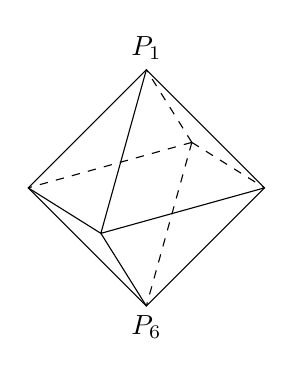
\begin{tikzpicture}[scale=1.5]
% Octahedron
\coordinate (A) at (1,0,0);
\coordinate (B) at (0,1,0);
\coordinate (C) at (-1,0,0);
\coordinate (D) at (0,-1,0);
\coordinate (E) at (0,0,1);
\coordinate (F) at (0,0,-1);
\draw (A) -- (B) -- (C) -- (D) -- cycle;
\draw (E) -- (A) (E) -- (B) (E) -- (C) (E) -- (D);
\draw[dashed] (F) -- (A) (F) -- (B) (F) -- (C) (F) -- (D);
\node[above] at (B) {$P_1$};
\node[below] at (D) {$P_6$};
\end{tikzpicture}
\end{center}

[解2] 正八面体の中心を $O$ とし、$\overrightarrow{OX} = \vec{v}$ となる点 $X$ をとる。$P_1, \cdots, P_6$ の中で点 $X$ から最も近い点を $P_k$ とする。$\overline{P_k X} \le \overline{P_m X}$ より
\[ |\overrightarrow{OX} - \overrightarrow{OP_k}| \le |\overrightarrow{OX} - \overrightarrow{OP_m}| \]
各辺 $0$ 以上だから $2$ 乗して
\begin{eqnarray*}
2 (\overrightarrow{OP_m} - \overrightarrow{OP_k}) \cdot \overrightarrow{OX} &\le& |\overrightarrow{OP_m}|^2 - |\overrightarrow{OP_k}|^2 = 0 \\
\therefore \overrightarrow{P_k P_m} \cdot \vec{v} &\le& 0
\end{eqnarray*}
$\overrightarrow{P_k P_m} \cdot \vec{v} \neq 0$ から
\[ \overrightarrow{P_k P_m} \cdot \vec{v} < 0 \]

\subsection*{第5問}
[解] (1) から $|z_k|^p = 1 \ \therefore |z_k| = 1 \cdots \text{\textcircled{1}}$。又 $z_k \neq 1 \cdots \text{\textcircled{2}}$
\textcircled{1}、\textcircled{2}から $z_k = \cos\theta + i\sin\theta\ (0 < \theta < 2\pi)$ とおくと、$z_k = e(i\theta_k)\ (0 < \theta_k < 2\pi)$ とおける。(イ)、(ロ)から
\begin{eqnarray*}
\begin{cases} e(p\theta_k) = 1 \\ e(\frac{2\pi}{p}\theta_k) = 1 \end{cases} \cdots \text{\textcircled{3}}
\end{eqnarray*}
したがって、\textcircled{3}を満たす $\{\theta_k\}$ の個数が $a_n$ である。\textcircled{3}の第1式から、適当な自然数 $m_k$ を用いて
\[ \theta_k = \frac{2\pi}{p}m_k\ (m_k = 1, 2, \cdots, p-1) \cdots \text{\textcircled{4}} \]
とおける。したがって、$\{\theta_k\}$ の個数は $\{m_k\}$ の数に他ならない。\textcircled{3}の第2式に\textcircled{4}を代入して整理して、
\[ \frac{2\pi}{p} m_k \equiv 0 \pmod p \cdots \text{\textcircled{5}} \]
又、題意の $n$ を $n \in \mathbb{N}$ に拡張してかんがえる。
\[ a_1 = 0,\ a_2 = p-1,\ a_3 = (p-1)(p-2) \cdots (1) \]
(2) $S_n = \sum_{k=1}^n m_k$ とおく。$m_k = 1, 2, \cdots, p-1$ から
\[ \begin{cases} S_n \equiv 0 \pmod p \text{ の時、} S_{n+1} \not\equiv 0 \\ S_n \not\equiv 0 \pmod p \text{ の時、対応する } m_{n+1} \text{ がただ } 1 \text{ つあって、} S_{n+1} \equiv 0 \text{ となる。} \end{cases} \]
$S_n$ の値のとり方は、$(p-1)^n$ 通りだからしたがって、$S_n \equiv 0$ となる場合の数は
\[ a_{n+1} = (p-1)^n - a_n \]
(3) $b_n = \frac{a_n}{(p-1)^n}$ とおく。(2)から
\begin{eqnarray*}
b_{n+1} &=& -\frac{1}{p-1} b_n + \frac{1}{p-1} \\
b_{n+1} - \frac{1}{p} &=& -\frac{1}{p-1} \left(b_n - \frac{1}{p}\right)
\end{eqnarray*}
$b_1=0$ だから、くり返し用いて、
\begin{eqnarray*}
b_n &=& \left(-\frac{1}{p-1}\right)^{n-1} \left(-\frac{1}{p}\right) + \frac{1}{p} \\
a_n &=& \frac{1}{p} \left[ (p-1)^n + (-1)^n (p-1) \right]
\end{eqnarray*}

[解2] (法$p$とする)
(2) $a_{n+2}$ についてかんがえる。
$1^\circ\ m_{n+1} + m_{n+2} \equiv 0$ の時
このような $(m_{n+1}, m_{n+2})$ のくみあわせは $1 \le m_i \le p-1$ から、$m_{n+1}$ を定めればただ $1$ 通りに定まり、$p-1$ 通り。又、$S_{n+2} \equiv 0 \iff S_n \equiv 0$ だから、$m_1 \sim m_n$ の定め方は $a_n$ 通り。あわせて
\[ (p-1) a_n \text{ 通り} \]
$2^\circ\ m_{n+1} + m_{n+2} \equiv r\ (r=1, 2, \cdots, p-1)$ の時
$m_{n+1}$ のえらび方は $1, 2, \cdots, p-1$ から $r$ をのぞいた $p-2$ 通り。
$m_{n+2}$ は、
\begin{eqnarray*}
m_{n+1} < r \text{ ならば } m_{n+2} &=& r - m_{n+1} \\
m_{n+1} > r \text{ ならば } m_{n+2} &=& p + r - m_{n+1}
\end{eqnarray*}
と各々 $1$ 通りに定まる。又、$S_{n+2} \equiv 0 \iff S_n + r \equiv 0$ だから、$m_1 \sim m_n$ の定め方は $a_{n+1}$ 通り。あわせて
\[ (p-2) a_{n+1} \]
以上で全ての場合がつくされ、$1^\circ, 2^\circ$ は排反だから
\[ a_{n+2} = (p-2)a_{n+1} + (p-1)a_n \]

\subsection*{第6問}
[解] $k \in \mathbb{N}$ に対し、$a_k = \int_{\frac{k-1}{n}\pi}^{\frac{k}{n}\pi} e^{-x} |\sin nx| dx$ とおく。$A_n = \int_0^\pi e^{-x} |\sin nx| dx$
おくと、
\[ A_n = \sum_{k=1}^n a_k \cdots \text{\textcircled{1}} \]
である。
\begin{eqnarray*}
a_{k+1} &=& \int_{\frac{k}{n}\pi}^{\frac{k+1}{n}\pi} e^{-x} |\sin nx| dx \\
&=& \int_{\frac{k-1}{n}\pi}^{\frac{k}{n}\pi} e^{-(t+\frac{\pi}{n})} |\sin n(t+\frac{\pi}{n})| dt\ (t = x - \frac{\pi}{n}) \\
&=& e^{-\frac{\pi}{n}} a_k \cdots \text{\textcircled{2}}
\end{eqnarray*}
又、
\begin{eqnarray*}
a_1 &=& \int_0^{\frac{\pi}{n}} e^{-x} \sin nx dx \\
&=& \left[ \frac{e^{-x}}{1+n^2} (-\sin nx - n \cos nx) \right]_0^{\frac{\pi}{n}} \\
&=& \frac{1}{1+n^2} \{ e^{-\frac{\pi}{n}} (n) - 1(-n) \} \\
&=& \frac{n}{1+n^2} (e^{-\frac{\pi}{n}} + 1) \cdots \text{\textcircled{3}}
\end{eqnarray*}
だから \textcircled{2} をくり返し用いて、
\[ a_k = e^{-\frac{(k-1)}{n}\pi} a_1 \]
\textcircled{1} に代入して
\begin{eqnarray*}
A_n &=& \sum_{k=0}^{n-1} a_1 e^{-\frac{k}{n}\pi} \\
&=& a_1 \frac{1-e^{-n \frac{\pi}{n}}}{1-e^{-\frac{\pi}{n}}} = \frac{n}{1+n^2} (1+e^{-\frac{\pi}{n}}) \frac{1-e^{-\pi}}{1-e^{-\frac{\pi}{n}}} \\
&=& \frac{n}{1+n^2} \frac{\frac{\pi}{n}}{1-e^{-\frac{\pi}{n}}} \left(\frac{1}{\frac{\pi}{n}}\right) (1+e^{-\frac{\pi}{n}})(1-e^{-\pi}) \\
&=& \frac{1}{1+\frac{1}{n^2}} \frac{\frac{\pi}{n}}{1-e^{-\frac{\pi}{n}}} (1-e^{-\pi}) \left(\frac{1}{\pi}\right) (1+e^{-\frac{\pi}{n}}) \\
&\xrightarrow{n\to\infty}& 1 \cdot 1 \cdot (1-e^{-\pi}) \cdot \left(\frac{1}{\pi}\right) \cdot 2 = \frac{2}{\pi}(1-e^{-\pi})
\end{eqnarray*}

[解2] (\textcircled{1} まで同じ)
$[\frac{k-1}{n}\pi, \frac{k}{n}\pi]$ において、$e^{-\frac{k}{n}\pi} \le e^{-x} \le e^{-\frac{k-1}{n}\pi}$ だから、$|\sin nx| \ge 0$ とあわせて、
\[ e^{-\frac{k}{n}\pi} \int_{\frac{k-1}{n}\pi}^{\frac{k}{n}\pi} |\sin nx| dx \le a_k \le e^{-\frac{k-1}{n}\pi} \int_{\frac{k-1}{n}\pi}^{\frac{k}{n}\pi} |\sin nx| dx \]
\[ \frac{2}{n} e^{-\frac{k}{n}\pi} \le a_k \le \frac{2}{n} e^{-\frac{k-1}{n}\pi} = e^{\frac{\pi}{n}} \left( \frac{2}{n} e^{-\frac{k}{n}\pi} \right) \cdots \text{\textcircled{2}} \]
ここで、$B_n = \sum_{k=1}^n \frac{2}{n} e^{-\frac{k}{n}\pi}$ とすると、
\[ B_n = \frac{2}{n} e^{-\frac{\pi}{n}} \frac{1-e^{-\pi}}{1-e^{-\frac{\pi}{n}}} \]
だから \textcircled{1}、\textcircled{2} より、
\[ B_n \le A_n \le e^{\frac{\pi}{n}} B_n \]
はさみうちから
\[ A_n \to B_n \]
で、
\[ B_n = \frac{\frac{\pi}{n}}{1-e^{-\frac{\pi}{n}}} \frac{2}{\pi} e^{-\frac{\pi}{n}} (1-e^{-\pi}) \to \frac{2}{\pi}(1-e^{-\pi}) \]
から
\[ A_n \to \frac{2}{\pi}(1-e^{-\pi}) \]

\end{document}
